\documentclass[fleqn,reqno,10pt]{article}

\usepackage{myarticlestyledefault}

\usepackage{pgfplots}

\begin{document}

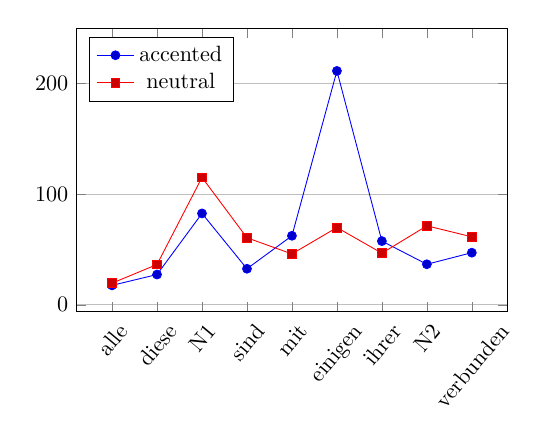
\begin{tikzpicture}[scale=0.8]
  \begin{axis}[
    legend pos = north west,
    ymajorgrids,
    ymax = 250,
    y = 0.5,
    x tick label style = {rotate = 50},
    xtick = data,
    xticklabels = {alle,diese,N1,sind,mit,einigen,ihrer,N2,verbunden}
    ]
    \addplot coordinates {
      (0 ,17.6)
      (1 ,27.4)
      (2 ,82.6)
      (3 ,32.6)
      (4 ,62.4)
      (5 ,211.3333333)
      (6 ,57.6)
      (7 ,36.66666667)
      (8 ,47.13333333)};

  \addplot coordinates {
        (0 ,19.6        )
        (1 ,36.46666667 )
        (2 ,115.1333333 )
        (3 ,60.6        )
        (4 ,46          )
        (5 ,69.86666667 )
        (6 ,46.66666667)
        (7 ,71.4)
        (8 ,61.46666667)};

      \legend{accented, neutral}


  \end{axis}
\end{tikzpicture}


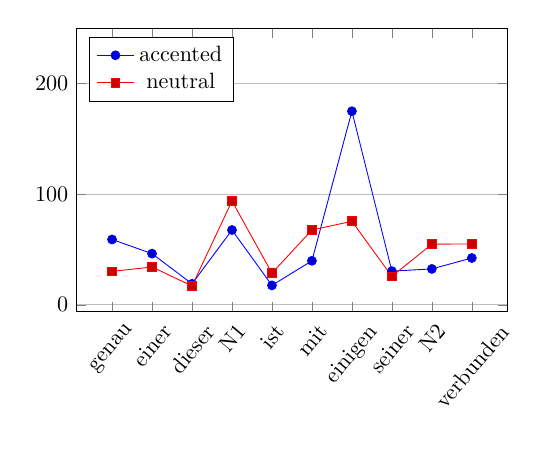
\begin{tikzpicture}[scale=0.8]
  \begin{axis}[
    legend pos = north west,
    ymajorgrids,
    ymax = 250,
    y = 0.5,
    x tick label style = {rotate = 50},
    xtick = data,
    xticklabels = {genau,einer,dieser,N1,ist,mit,einigen,seiner,N2,verbunden}
    ]
    \addplot coordinates {
        (     0 , 59.06666667 )
        (     1 , 46.26666667 )
        (     2 , 19          )
        (     3 , 67.6        )
        (     4 , 17.6        )
        (     5 , 39.8        )
        (     6 , 174.9333333 )
        (     7 , 30.46666667 )
        (     8 , 32.46666667 )
        (     9 , 42.33333333 )};

  \addplot coordinates {
        (0 , 30.21428571 )
        (1 , 34.21428571 )
        (2 , 17.07142857 )
        (3 , 93.78571429 )
        (4 , 28.64285714 )
        (5 , 67.64285714 )
        (6, 75.5        )
        (7 , 25.71428571 )
        (8 , 54.85714286 )
        (9 , 55)};

      \legend{accented, neutral}


  \end{axis}
\end{tikzpicture}


\end{document}
